\documentclass[a4paper,11pt]{article}
\usepackage[czech]{babel}
\usepackage[margin=2cm]{geometry}
\usepackage{graphicx}
\usepackage{hyperref}
\hypersetup{hidelinks}
\usepackage{float}

\begin{document}

\begin{titlepage}
\centering

% logo - odkomentuj, až ho nahraješ (viz níže)

\includegraphics[width=0.6\textwidth]{pictures/logo_cz.png}

\vspace{\stretch{0.382}}

{\Huge Projektová dokumentace\par}
\vspace{0.3em}
{\Large\bfseries Implementace překladače jazyka IFJ26\par}
\vspace{0.3em}
{\large Tým xhanzlp00, varianta vv-BVS\par}

\vspace{1.5em}
Rozšíření: \texttt{FUNEXP}, \texttt{BOOLTHEN}, \texttt{CONTROL}, \texttt{VALMEM}, \texttt{LISTS}, \texttt{PARAMLISTS}\par
Repozitář: \url{https://github.com/HanzlikPetr/IFJ26}

\vspace{\stretch{0.618}}

\begin{minipage}[b]{0.3\textwidth}
\raggedright\large
27. listopadu 2026
\end{minipage}
\hfill
\begin{minipage}[b]{0.68\textwidth}
\raggedleft\large
\begin{tabular}{llll}
\textbf{Petr Hanzlík} & \textbf{(xhanzlp00)} & \textbf{282000} & 25\,\% \\
Vojtěch Jurok & (xjurokv00) & 281890 & 25\,\% \\
Ondřej Glet & (xgleton00) & 282467 & 25\,\% \\
Marek Beran & (xberanm00) & 282821 & 25\,\% \\
\end{tabular}
\end{minipage}

\end{titlepage}

\newpage

\section{Rozdělení práce}

\begin{itemize}
  \item \textbf{Petr Hanzlík} -- \texttt{Makefile} a CI, implementace
        výškově vyváženého stromu, tabulka symbolů, sémantická analýza,
        prezentace, PSA
  \item \textbf{Vojtěch Jurok} -- lexikální analýza, dynamické struktury,
        systémové testy, diagram konečného automatu, dokumentace
  \item \textbf{Ondřej Glet} -- LL gramatika a LL tabulka, syntaktická analýza,
        implementace AST, systémové testy
  \item \textbf{Marek Beran} -- implementace zásobníku, blokové schéma
        architektury, generátor cílového kódu
\end{itemize}

\noindent Každý člen týmu psal jednotkové testy ke svým modulům.

\section{Spolupráce, testování a styl kódu}

\begin{itemize}
  \item \textbf{Spolupráce:}
    \begin{itemize}
      \item Tým komunikoval průběžně přes Discord a na společných přednáškách.
      \item Vývoj probíhal na GitHubu ve vlastních větvích a změny jsme
            začleňovali do větve \texttt{main} přes pull requesty (PR).
      \item Měli jsme předem dané, kdo bude komu dělat code review
            (Ondřej $\rightarrow$ Vojtěch,
            Petr $\rightarrow$ Ondřej, Marek $\rightarrow$ Petr,
            Vojtěch $\rightarrow$ Marek).
      \item Podmínkou pro sloučení PR bylo schválení od člověka, který dělal review
            a úspěšný průchod CI pipeline, která kontrolovala build,
            formátování kódu a spouštěla testy včetně kontroly paměti.
      \item Pro udržení čisté a lineární historie jsme k mergování
            využívali rebase.
    \end{itemize}
  \item \textbf{Testování:}
    \begin{itemize}
      \item Jednotkové testy: jednotlivé části kódu jsme testovali v cmocka
            a pomocí Valgrindu u nich rovnou kontrolovali paměťové chyby.
      \item Systémové testy: ve složce \texttt{tests/data} jsou připravené
            zdrojové kódy v jazyce IFJ26. Ty automaticky překládáme
            a zjišťujeme, jestli se jejich skutečný výstup a návratový kód
            shoduje s očekávaným.
    \end{itemize}
  \item \textbf{Styl kódu:} zvolili jsme styl LLVM. Kód formátujeme nástrojem
        \texttt{clang-format} a správné formátování u každé změny
        automaticky kontroluje CI.
\end{itemize}
\newpage
\section{Architektura překladače}

\newpage
\section{Lexikální analýza}
Konečný automat lexikálního analyzátoru je na obrázcích~\ref{fig:ka1}
a~\ref{fig:ka2}, odchylky od standardního modelu jsou popsány pod nimi.

\begin{figure}[H]
  \centering
  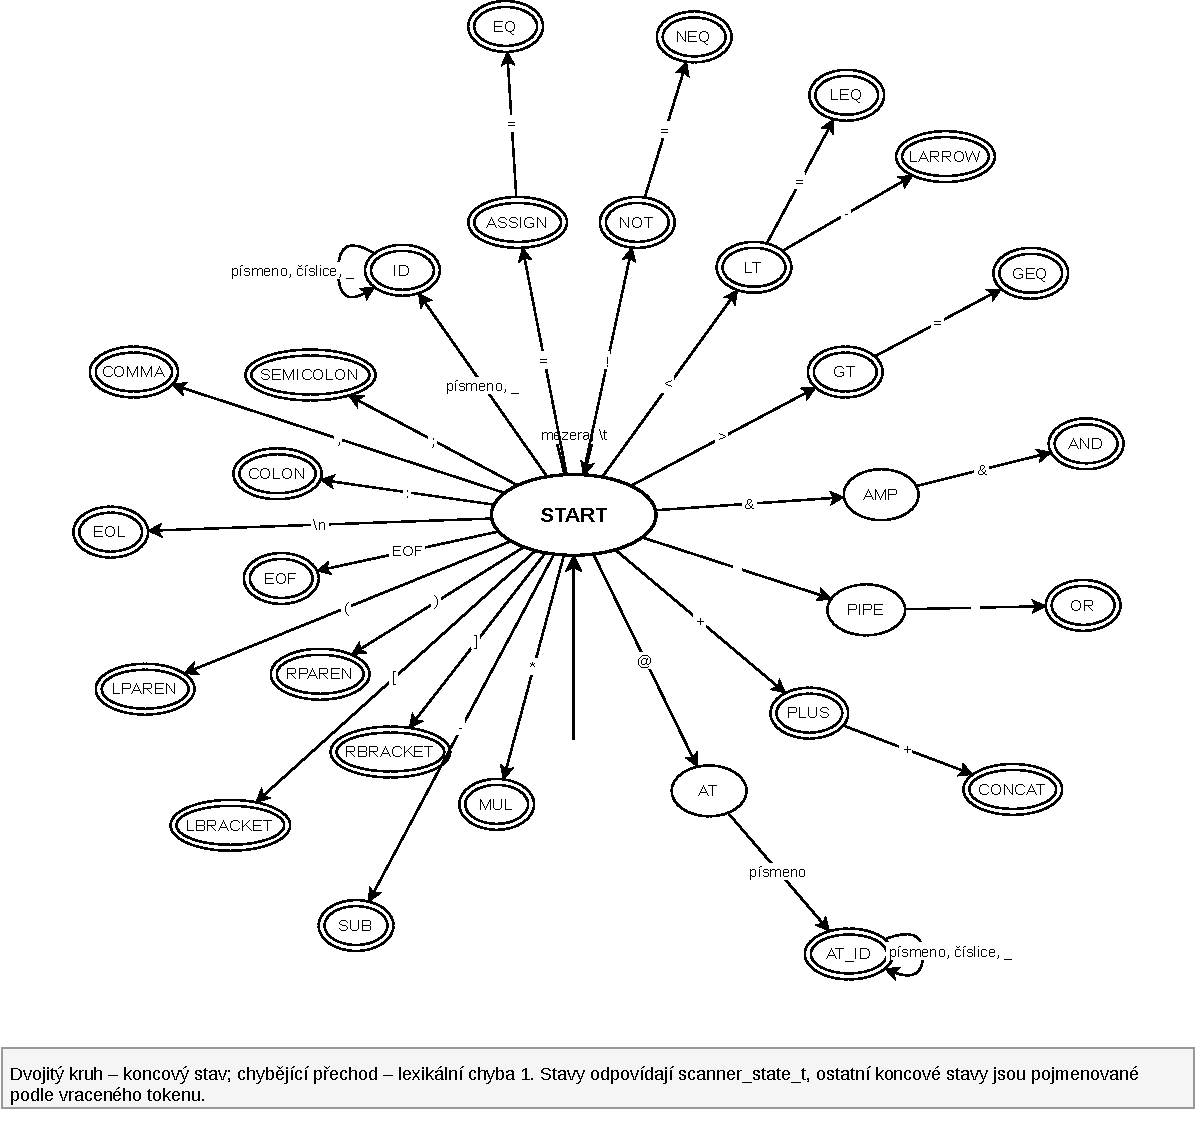
\includegraphics[page=1,width=\textwidth,height=0.85\textheight,keepaspectratio]{pictures/automat3.pdf}
  \caption{Konečný automat lexikálního analyzátoru -- identifikátory, operátory a oddělovače}
\label{fig:ka1}
\end{figure}
\clearpage

\begin{figure}[H]
  \centering
  \includegraphics[page=2,width=\textwidth,height=0.9\textheight,keepaspectratio]{pictures/automat3.pdf}
  \caption{Konečný automat lexikálního analyzátoru -- čísla, řetězce a komentáře}
\label{fig:ka2}
\end{figure}
\clearpage
\textbf{Odchylky od standardního konečného automatu:}
    \begin{itemize}
        \item Znak nepatřící do tokenu se přes \texttt{ungetc} vrací pro další cyklus (stav \texttt{START}).
        \item \texttt{ID}: lexém se porovná s tabulkou klíčových slov (shoda → \texttt{KEYWORD})
        \item Úroveň mezer na začátku řádku porovnáváme se zásobníkem a generujeme příslušné tokeny \texttt{INDENT/DEDENT}.
        \item Token \texttt{EOL} se v závorkách a na prázdných řádcích nevydává.
      Na konci souboru se vydá \texttt{EOL}, všechny zbývající
      \texttt{DEDENT}y a nakonec \texttt{EOF}.
\item Zanoření blokových komentářů hlídáme pomocí počítadla, takže automat
      už není čistě konečný. Pokud komentář obsahuje znak nového řádku,
      chová se pro zbytek překladače jako konec řádku, jinak jako mezera.
        \item Každý token si pamatuje, jestli mu předcházelo odřádkování, a to i uvnitř závorek, kde se \texttt{EOL} nevydává. Parser to potřebuje vědět, aby mohl správně povolit koncovou čárku před uzavírací závorkou.
        \item Funkce \texttt{scanner\_peek\_next\_token} umožňuje parseru podívat se na další token, aniž by ho rovnou spotřeboval.
    \end{itemize}
\section{Syntaktická analýza}
\newpage
\section{Popis modulů}

\begin{description}
  \item[\texttt{compiler.c}] Hlavní modul, který řídí celý překlad.
  Nechá parser
  sestavit abstraktní
  syntaktický strom (AST), zaregistruje všechny funkce do tabulky symbolů, spustí
  sémantickou kontrolu a generování kódu. Při chybě vrací příslušný
  chybový kód.
  \item[\texttt{scanner.c/h}] Modul funguje jako konečný automat, který čte zdrojový text ze standardního vstupu a přes funkce jako \texttt{scanner\_next\_token} předává parseru zpracované tokeny. Pro sledování úrovní odsazení využívá datovou strukturu zásobníku z modulu \texttt{stack}.
  \item[\texttt{dstring.c/h}] Modul implementuje dynamický řetězec, který se podle potřeby sám zvětšuje. Scanner v něm postupně skládá lexémy, u kterých předem nezná jejich délku.
\item[\texttt{parser.c/h}] Pomocí rekurzivního sestupu postupně čte tokeny a rovnou z nich staví AST. Syntaktickou analýzu výrazů přenechává modulu \texttt{psa}.
\item[\texttt{psa.c/h}] Provádí precedenční syntaktickou analýzu výrazů
  a staví z nich AST, včetně volání funkcí a \texttt{if} výrazů. Výrazy
  s konstantami spočítá už při překladu (constant folding).
\item[\texttt{ast.c/h}] Poskytuje datovou strukturu uzlů AST, která využívá union a dynamická pole pro
  potomky. Vytvořený strom pak využívá sémantická analýza, která do uzlů
  doplňuje odvozené typy výrazů, a generátor kódu.
  \item[\texttt{semantic\_analy.c/h}] Pracuje ve dvou fázích -- nejdřív uloží
  signatury všech funkcí do tabulky symbolů, pak kontroluje jejich těla
  a zapisuje odvozené typy do AST. Lokální proměnné hlídá v~zásobníku tabulek
  symbolů (jedna pro každý blok) a pro generátor kódu jim přiděluje unikátní
  jména.
  \item[\texttt{symtable.c/h}] Tabulka symbolů postavená na AVL stromu, který je naimplementovaný přímo v tomto modulu. Zbytek překladače do ní podle identifikátoru jako klíče ukládá a vyhledává funkce i lokální proměnné.
\item[\texttt{stack.c/h}] Obecný zásobník implementovaný jako jednosměrně vázaný seznam, který díky ukazatelům \texttt{void *} dokáže uchovat libovolná data. Využívá ho scanner pro hlídání odsazení, PSA pro symboly výrazů a sémantická analýza pro ukládání lokálních tabulek symbolů.
  \item[\texttt{printer\_tree.c/h}] Modul pro názorný výpis struktury AST a doplněných typů. Slouží výhradně k~ladění a při překladu kódu se nijak nepoužívá.
\item[\texttt{error.h}] Definuje chybové kódy podle specifikace a makra pro
  jejich snadné předávání dál. Chybová hlášení vypisuje na \texttt{stderr}.
\end{description}









\newpage
\section{Využití AI}




\paragraph{Pracovní postup.}
Při vývoji jsme využívali Claude, Gemini, GitHub Copilot a OpenCode
s~modelem \mbox{GLM-5.3}.
AI nám sloužila především k vysvětlení nejasností v zadání či konceptech
jazyka C a k hledání chyb v už napsaném kódu.
Kód jsme pomocí AI generovali jen pro menší ohraničené úseky nebo testy podle
přesného popisu. Tyto části jsou ve zdrojovém kódu označené komentářem
s použitým promptem. Každý výstup od AI pak procházel stejným code review v PR
jako naše vlastní práce a musel projít jednotkovými testy včetně kontroly přes
Valgrind.

\paragraph{Kód vytvořený pomocí AI.}
Všechny tyto části jsou v kódu označeny komentářem včetně promptu.

\begin{center}
\begin{tabular}{lll}
\textbf{Soubor} & \textbf{Nástroj} & \textbf{Část} \\
\hline
\texttt{parser.c}, \texttt{psa.c} & OpenCode & \texttt{if} výraz (CONTROL) \\
\texttt{semantic\_analy.c} & GLM-5.3 (OpenCode) & kontroly LISTS, detekce rekurze \\
\texttt{printer\_tree.c} & Gemini, GLM-5.3 & ladicí výpis AST \\
\texttt{error.h} & Gemini 3.1 Pro & makro \texttt{CHECK\_ARGS\_NULL\_RET} \\
\texttt{symtable.c} & GLM-5.3 (OpenCode) & přesun \texttt{ifj26\_type2str} \\
\texttt{scanner.c} & Claude Opus 5.5 & převod stavu do struktury \texttt{scanner\_t} \\
\texttt{tests/utest/*} & Claude Opus 5.5 & jednotkové testy \\
\texttt{tests/system}, \texttt{tests/data} & Claude Opus 5.5 & systémové testy \\
\end{tabular}
\end{center}

\paragraph{Problémy a odmítnuté návrhy.}




\begin{itemize}
  \item Při psaní scanneru nám AI například navrhla, aby scanner rovnou hlásil lexikální chybu u zápisů
jako \texttt{1e5f} nebo \texttt{0x1F} a odmítl písmeno nalepené hned za číslem.
V materiálech k předmětu jsme ale zjistili, že automat má být „žravý“ a vrátit
to jako dva samostatné tokeny, takže chybu musí odhalit až parser. Návrh jsme
proto nepoužili.
  \item Při práci na sémantické analýze GitHub Copilot u delších bloků kódu ztrácel
kontext, proto jsme ho používali hlavně k doplňování názvů. Agenta
v OpenCode bylo občas potřeba usměrnit, aby neduplikoval existující kód --
například aby místo vlastní implementace využil již hotový obecný zásobník.
\end{itemize}

\end{document}
